\documentclass[12pt,-letter paper]{article}
\usepackage{siunitx}
\usepackage{setspace}
\usepackage{gensymb}
\usepackage{xcolor}
\usepackage{caption}
%\usepackage{subcaption}
\doublespacing
\singlespacing
\usepackage[none]{hyphenat}
\usepackage{amssymb}
\usepackage{relsize}
\usepackage[cmex10]{amsmath}
\usepackage{mathtools}
\usepackage{amsmath}
\usepackage{commath}
\usepackage{amsthm}
\interdisplaylinepenalty=2500
%\savesymbol{iint}
\usepackage{txfonts}
%\restoresymbol{TXF}{iint}
\usepackage{wasysym}
\usepackage{amsthm}
\usepackage{mathrsfs}
\usepackage{txfonts}
\let\vec\mathbf{}
\usepackage{stfloats}
\usepackage{float}
\usepackage{cite}
\usepackage{cases}
\usepackage{subfig}
%\usepackage{xtab}
\usepackage{longtable}
\usepackage{multirow}
%\usepackage{algorithm}
\usepackage{amssymb}
%\usepackage{algpseudocode}
\usepackage{enumitem}
\usepackage{mathtools}
%\usepackage{eenrc}
%\usepackage[framemethod=tikz]{mdframed}
\usepackage{listings}
%\usepackage{listings}
\usepackage[latin1]{inputenc}
%%\usepackage{color}{   
%%\usepackage{lscape}
\usepackage{textcomp}
\usepackage{titling}
\usepackage{hyperref}
%\usepackage{fulbigskip}   
\usepackage{tikz}
\usepackage{graphicx}
\lstset{
  frame=single,
  breaklines=true
}
\let\vec\mathbf{}
\usepackage{enumitem}
\usepackage{graphicx}
\usepackage{siunitx}
\let\vec\mathbf{}
\usepackage{enumitem}
\usepackage{graphicx}
\usepackage{enumitem}
\usepackage{tfrupee}
\usepackage{amsmath}
\usepackage{amssymb}
\usepackage{mwe} % for blindtext and example-image-a in example
\usepackage{wrapfig}
\graphicspath{{figs/}}
\providecommand{\mydet}[1]{\ensuremath{\begin{vmatrix}#1\end{vmatrix}}}
\providecommand{\myvec}[1]{\ensuremath{\begin{bmatrix}#1\end{bmatrix}}}
\providecommand{\cbrak}[1]{\ensuremath{\left\{#1\right\}}}
\providecommand{\brak}[1]{\ensuremath{\left(#1\right)}}

\title{Matrix assignment}
\date{\today}

\begin{document}

\maketitle{Questions}
\begin{enumerate}
	\item The pair of linear equations $ 2x=5y+6 $ and $ 15y=6x-18 $ represents two lines which are : 
\begin{enumerate}
    \item intersecting
    \item parallel
    \item coincident
    \item either intersecting or parallel
\end{enumerate}
\item Two schools $P$ and $Q$ decided to award prizes to their students for two games of Hockey \rupee $x$ per students and cricket \rupee $y$ per student. School $P$
decided to award a total of \rupee $9,500$ for the two games to $5$ and $4$ students respectively; while school $Q$ decided to award \rupee $7,370$ for the two games to $4$ and $3$ students respectively.
\begin{figure}[H]
    \centering
    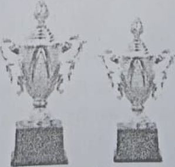
\includegraphics[width=\columnwidth]{figs/math.png}
    \caption{trophies}
    \label{fig:trophies}
\end{figure}


Based on the given information, answer the following questions :
\begin{enumerate}[label=(\roman*)]
    \item Represent the following information algebraically(in terms of $x$ and $y$).
    \item\begin{enumerate}[label=(\alph*)]
\item what is the prize amount for hockey ?
\item Prize amount on which game is more and by how much ?
    \end{enumerate}
    \item what will be the total prize amount if there are $2$ students each from two games ?
\end{enumerate}
\item If the pair of equations $3x - y + 8 = 0$ and $6x - ry +16 =0$ represents coincident lines,then the values of $r$ is :
\begin{enumerate}[label=(\alph*)]
    \item $-\frac{1}{2}$
    \item $\frac{1}{2}$
    \item $2$
    \item $-2$
\end{enumerate}
\item The pair of equations $x=a$ and $y=b$ graphically represents lines which are :
\begin{enumerate}[label=(\alph*)]
    \item parallel
    \item intersecting at $\brak{b,a}$
    \item coincident
    \item intersecting at $\brak{a,b}$
\end{enumerate}
\item
\begin{enumerate}[label=(\alph*)]
\item If the system of linear equations 
$2x + 3y = 7$  and   $2ax +\brak{a + b}y =28$ 
have infinite number of solutions, then find the values of $a$ and $b$.
\item  If $217x + 131y = 913$ and  
$131x + 217y = 827$,  then solve the equations for the values of $x$ and $y$.
\end{enumerate}
\item Half of the difference between two numbers is $2$. The sum of the greater number and twice the smaller number is $3$.Find the numbers.
\item If \brak{a,b},\brak{c,d} and \brak{e,f} are the vertices of $\triangle ABC$ and $\Delta$ denotes the area of $\triangle ABC$, then 
  \begin{align}
      \mydet{a & c & e\\b & d& f\\1&1&1}^2 
  \end{align}  
 is equal to
\begin{enumerate}[label=(\alph*)]
    \item 2$\Delta ^2$
    \item 4$\Delta ^2$ 
    \item 2$\Delta$
    \item 2$\Delta$
\end{enumerate}
    \item If $\myvec{2 & 0 \\5 & 4} = P + Q$ 
is a symmetric and $Q$ is a skew symmetric matrix, then $Q$ is equal to
\begin{enumerate}[label=(\alph*)]
    \item $\myvec{2  & \frac{5}{2} \\\frac{5}{2} & 4 }$
    \item $\myvec{ 0 & -\frac{5}{2} \\\frac{5}{2} & 0}$
    \item $\myvec{ 0 & \frac{5}{2} \\-\frac{5}{2} & 0}$
    \item $\myvec{2 & -\frac{5}{2} \\\frac{5}{2} & 4 }$
\end{enumerate}
\item If $\myvec{1 & 2 & 1 \\2 & 3 & 1 \\3 & a & 1}$
is non-singular matrix and  $a \in A $, then the set $A$ is 
\begin{enumerate}[label=(\alph*)]
    \item $\mathbb{R}$
    \item $\cbrak{0}$
    \item $\cbrak{4}$
    \item $\mathbb{R}-\cbrak{4}$
\end{enumerate}
\item If$\mydet{A} = \mydet{ kA}$, where $A$ is a square matrix of order $2$,then sum of all possible values of $k$ is
\begin{enumerate}[label=(\alph*)]
    \item $1$
    \item $-1$
    \item $2$
    \item $0$
\end{enumerate}
\item\begin{enumerate}[label=(\alph*)]
    \item If $A=\myvec{ -3 & -2 & -4\\2 & 1 & 2\\2 & 1 & 3}$
and $B =\myvec{  1 & 2 & 0\\-2 & -1 & -2\\0 & -1 & 1}$,then find $AB$ and use it to solve the following system of equations :
\begin{align} x - 2y &= 3\\2x - y - z &= 2\\-2y + z &= 3\end{align}
\item If $f\brak{\alpha}=\myvec{
    \cos\alpha & -\sin\alpha & 0\\
    \sin\alpha & \cos\alpha & 0\\
    0 & 0 & 1}$
 ,then prove that\begin{align}
      f\brak{\alpha}.f\brak{-\beta} =f\brak{(\alpha - \beta)}.
 \end{align}
\end{enumerate}
 \end{enumerate}
\end{document}
